\section{Kontext- und Typeinschränkungen}
\label{sec:constraints}
In den folgenden Kapitel werden die nötigen Kontext Checks beschrieben und 
deren Notwendigkeit erleutert.

\subsection{}

Beschreiben welche statischen Analysen Implementiert werden konnent/Probleme/usw.\\
\\
- Kontrolle ob Purness eingehalten\\
- Kontrolle ob conditions offensichtlich verletzt\\
(- evtl. Ableiten von conditions)


%\newpage

%\begin{figure*}[h]
%	\begin{center}
%		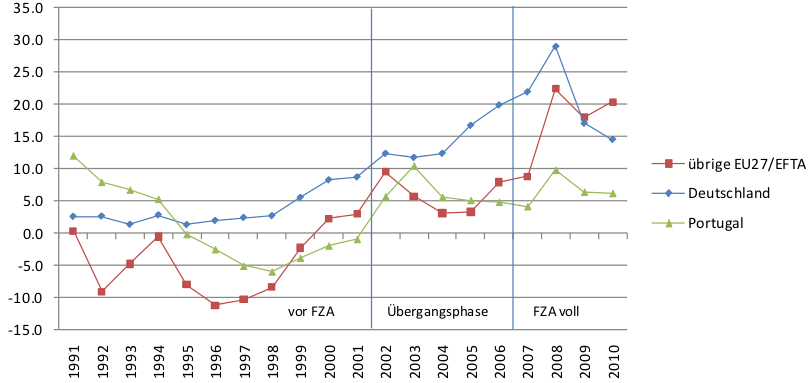
\includegraphics[width=0.9\textwidth]{images/Zuwanderungssaldo_Bericht_2.png}
%	\end{center}
%	\caption{Verlauf der Zuwanderung nach Herkunftsländern in Tausend \cite[S. 18]{ADMIN:Bericht}}
%	\label{fig:zuwanderungsaldi}
%\end{figure*}

